\documentclass[11pt,a4paper]{article}
\usepackage{amsmath,amssymb,calc,ifthen}
\usepackage{float}
%\usepackage{cancel}
\usepackage[table,usenames,dvipsnames]{xcolor} % for coloured cells in tables
\usepackage{tikz}
% Allows us to click on links and references!
\usepackage{hyperref}
\usepackage{url}
\hypersetup{
colorlinks,
citecolor=black,
filecolor=black,
linkcolor=black,
urlcolor=black
}
% Nice package for plotting graphs
% See excellent guide:
% http://www.tug.org/TUGboat/tb31-1/tb97wright-pgfplots.pdf
\usetikzlibrary{plotmarks,shapes}
\usepackage{amsmath,graphicx}
\usepackage{mathtools}
\usepackage{epstopdf}
\usepackage{caption}
\usepackage{subcaption}
\usepackage{graphicx}
% highlight - useful for TODOs and similar
\usepackage{color}
\newcommand{\hilight}[1]{\colorbox{yellow}{#1}}
\newcommand\ci{\perp\!\!\!\perp} % perpendicular sign
\newcommand*\rfrac[2]{{}^{#1}\!/_{#2}} % diagonal fraction
\newcommand\SLASH{\char`\\}
\usepackage{listings}
% margin size
\usepackage[margin=0.5in]{geometry}
\usepackage{pdfpages}
\usepackage{enumitem} % for nested enumerate numbers 1 1.1 1.1.1

\usepackage{titlesec} % reduce spacing after subsections

% \titlespacing\subsection{0pt}{4pt plus 4pt minus 2pt}{4pt plus 2pt minus 2pt}

\DeclareMathOperator*{\argmin}{arg\,min}
\DeclareMathOperator*{\argmax}{arg\,max}

\begin{document}
\belowdisplayskip=12pt plus 3pt minus 9pt
\belowdisplayshortskip=7pt plus 3pt minus 4pt


% \rowcolors{2}{gray!25}{white}


% \begin{figure}[H]
% \centering
% \includegraphics[scale=0.5]{../code/synthetic/14/figures/liksTrueFittedParams}
% \caption{14 clear biomk}
% \end{figure}
% 
% \begin{figure}[H]
% \centering
% \includegraphics[scale=0.5]{../code/synthetic/14/figures/liksTrueFittedParams}
% \caption{11 clear + 3 unclear biomk}
% \end{figure}


\definecolor{blue3}{HTML}{86B7FC} % med blue
\definecolor{blue1}{HTML}{B5F1FF} % light blue
\definecolor{blue2}{HTML}{E0F9FF} % very light blue

% \section{Motivation}
% 
% It is currently believed that neurodegenerative diseases target specific brain networks (Seeley, 2009). Moreover, different symptoms assiciated with different syndromes are thus believed to be a result of different underlying brain areas being affected. 

% TITLE Disease Knowledge Transfer for Alzheimer's Variants


\section{Abstract}

We present Disease Knowledge Transfer (DKT), a technique for transferring biomarker correlations between Alzheimer's disease (AD) variants. DKT allows, for the first time, to infer biomarker values and their progressions in rare variants of AD for which data on such biomarkers is not available, by learning them from a different disease. For doing this, we formulate a new dementias paradigm called "Affected Overlap", which proposes that dementias are diseases that affect overlapping brain regions, and thus present certain biomarker characteristics that are shared and can thus be transferred across diseases. We then formulate the DKT model implementing this paradigm as a joint-disease generative model of biomarker progression which disentangles the biomarker correlations that are disease-specific from those correlations that are disease-agnostic. We demonstrate DKT on three datasets: (1) the TADPOLE Challenge dataset containing typical AD subjects (tAD) from the Alzheimer's Disease Neuroimaging Initiative (ADNI) dataset who had MRI, FDG, AV45, AV1451 or DTI scans, as well as two datasets from our local centre containing subjects with (2) typical AD and (3) Posterior Cortical Atrophy (PCA) that have only undergone MRI scans. We train the DKT model on all three datasets at once, and show that it is able to predict, in PCA subjects, plausible population-level biomarker for FDG, DTI, AV45 and AV1451 biomarkers, for which no data was available. We validate the predictions of DKT using a small set of DTI scans for the PCA cohort. Finally, DKT can be a useful tool to analyse and understand rare forms of dementias for which multimodal data is not available or is limited (e.g. cross-sectional). Finally, by leveraging data from multiple diseases, DKT also has the potential to provide more accurate disease staging compared to traditional disease progression models, which is useful for patient stratification in clinical trials.


% 1. Statement of Novelty/Impact *

We present a novel dementias paradigm (Affected Overlap) and technique (DKT) that can be used to predict, for the first time, the population-level progression of biomarkers in a disease for which no such biomarker data is available, by transferring them from a different disease where they are available.



\section{Hierarchical model of disease progression}

The framework/model assumes that within a dataset of patients with a particular form of dementia, there are certain correlations between biomarkers that are \emph{disease agnostic}. For example, atrophy in the temporal lobe usually correlates with amyloid/tau-levels within the same region or with memory impairment. This is because we believe that amyloid/tau deposition cause neurodegeneration, which then causes cognitive decline in functions related to the underlying affected areas. One can then view different neurodenegenerative diseases as affecting a different set of brain regions and their underlying connectivity networks, a view supported by previous studies (Seeley, 2009, Zhou 2012). This view suggests that one can uniquely define a disease in terms of the different subset of brain regions that it affects. However, sometimes there are \emph{digo dktseasesease-agnostic} correlations that are not confined to a single region, e.g. disconnected brains regions are known to be responsible for certain cognitive functions, or biomarker measurements in different brain regions could correlate due to underlying structural or functional connectivity. One can therefore extend the idea of disease-agostic correlations between biomarkers to region-nonspecific sets of biomarkers which we will call \emph{functional units}, because the biomarkers being related through similar function.

We propose a hierarchical model of disease progression that disentangles \emph{disease-specific} biomarker correlations from \emph{disease-agnostic} correlations. For modelling disease-agnostic correlations, we assume biomarkers are grouped into \emph{functional units}, where corelations within each unit are disease-agnostic (e.g. biomarkers corresponding to the same ROI).  Each biomarker is assigned a-priori to a specific functional unit, which corresponds to a brain region, say temporal lobe (Fig 1., bottom).  For example, biomarkers assigned to the temporal unit could be: amyloid in temporal lobe, tau in temporal lobe, MRI atrophy in temporal lobe and certain memory tests. Using a disease progression model of our choice, for each region-specific functional unit we can model the correlation of biomarkers within that functional unit (Figure 1, bottom), which allows us to reconstruct a region- or unit-specific \emph{dysfunction} progression axis which can be used for staging subjects. Finally, we express the disease specific correlations (Figure 1, top) not directly with each biomarkers, but via the dysfunction scores estimated within each functional unit.  

The proposed model is parsimonious, easily interpretable by abstracting away biomarker information intothe functional units, and can be used for \emph{disease knowledge transfer}, i.e. learning correlations in one disease from another. Our approach is inspired by transfer learning methods from machine learning, but the model is generative, easing interpretability.   


\begin{figure}[h]
 \centering
 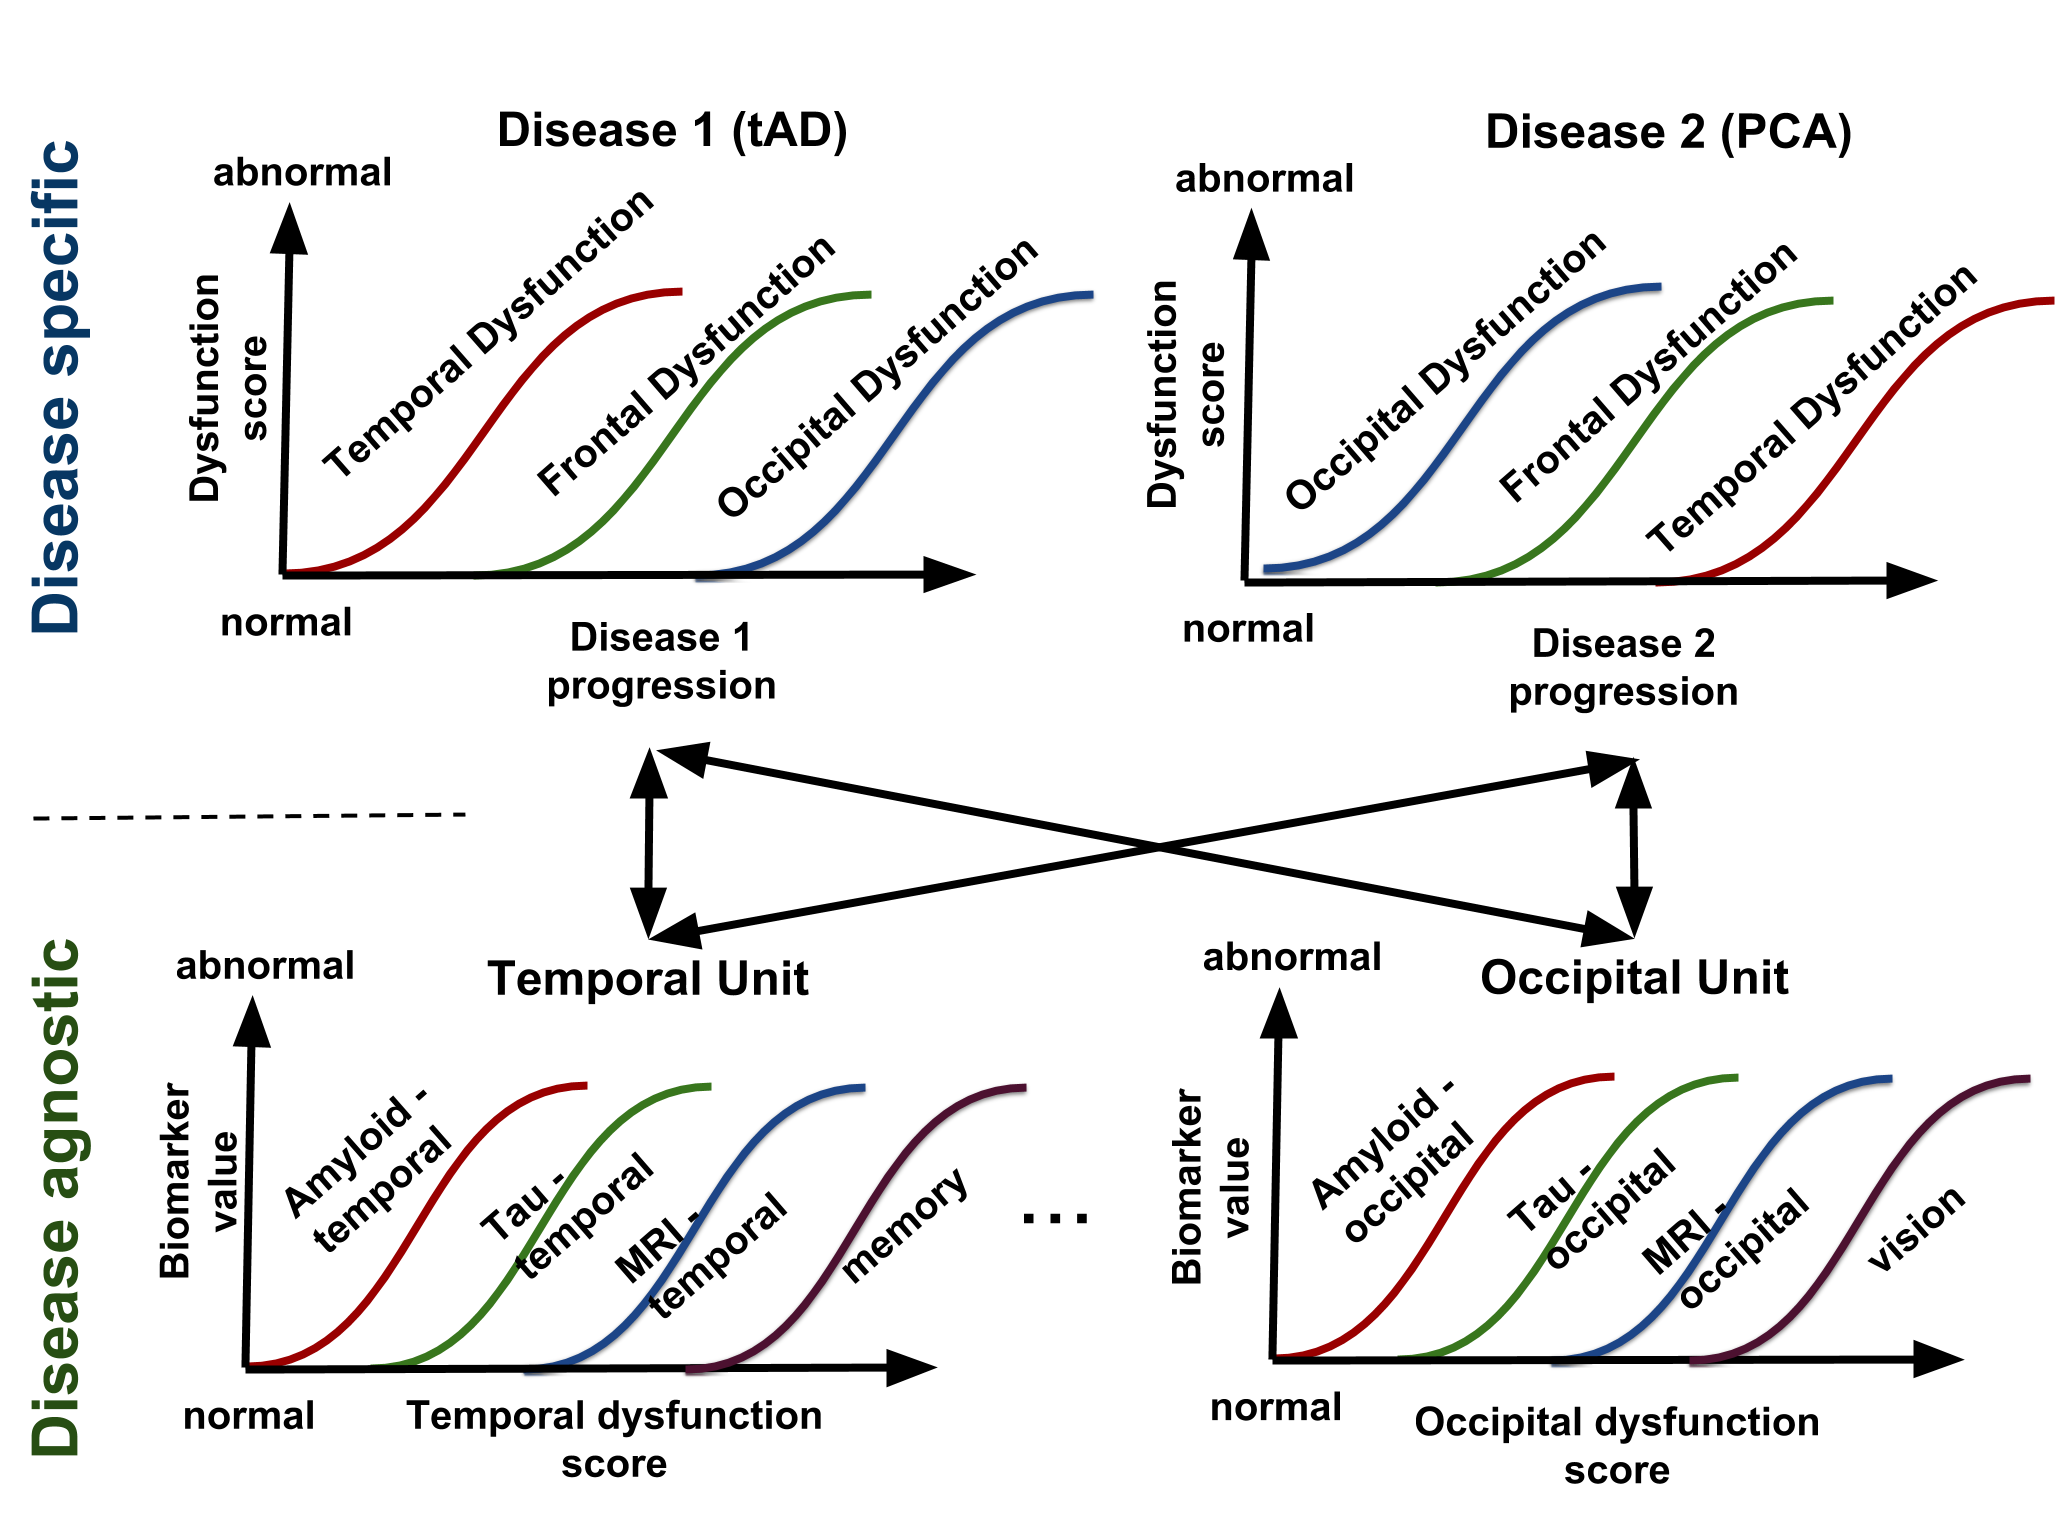
\includegraphics[height=11cm]{figures/disease_knowledge_transfer.png}
 \caption{Outline of the proposed framework for joint modelling of multiple diseases. }
\end{figure}

\subsection{Mathematical formulation}

Variable names:
\begin{itemize}
 \item $\Lambda$ = set of \emph{functional units}, i.e. \{temporal, parietal, occipital, ..\}. Biomarkers belonging to the same functional unit are asusmed to have disease-agnostic correlations.
 \item $y_{ijk}$ = measurement in subject $i$, visit $j$, biomarker $k$
%  \item $d_{ijl}$ = dysfunctionality score in subject $i$, visit $j$ in \emph{functional unit} $l$, where $l \in \Lambda$
%  \item $s_{ij}$ = disease progression score in subject $i$, visit $j$
 \item $\theta_k$ = parameters of trajectory for biomarker $k$
 \item $\lambda^l$ = parameters of trajectory for functional unit $l$, where $l \in \Lambda$
 \item $\psi$ : \{1, ..., K\} $ \rightarrow Lambda$ is a function that maps beach biomarker to its corresponding functional unit
 \item $\beta_i$: time shift parameter for subject $i$ (disease specific)
 \item $\beta_i^{l}$: time shift parameter for subject $i$ used in functional unit $l$, where $l \in \Lambda$
 \item $\Omega$: set ${(i,j,k)}$ of measurements available from every subject $i$, visit $j$ in biomarker $k$
\end{itemize}

Likelihood for one single measurement in one subject visit: 
\begin{equation}
 p(y_{ijk}|\theta_k, \lambda^{\psi(k)}, \beta_i) = \sum_{\beta_i^{\psi(k)}} p(y_{ijk}| \beta_i^{\psi(k)}, \theta_k) p(\beta_i^{\psi(k)}| \lambda^{\psi(k)}, \beta_i)
\end{equation}

where $\beta_i^{\psi(k)}$ is a latent variable denoting the stage of subject $i$ in functional unit $\psi(k)$, where biomarker $k$ was assigned.

Extending the above to multiple, subjects, visits and biomarkers, we get the final model likelihood:
\begin{equation}
 p(y_{.,.,.}|\theta_1, ..., \theta_K, \{\lambda^{\psi(l)} | l \in \Lambda \}, \beta_1, ..., \beta_N) = \prod_{(i,j,k) \in \Omega} \sum_{\beta_i^{\psi(k)}} p(y_{ijk}| \beta_i^{\psi(k)}, \theta_k) p(\beta_i^{\psi(k)}| \lambda^{\psi(k)}, \beta_i)
\end{equation}

Modelling of $p(y_{ijk}| \beta_i^{\psi(k)}, \theta_k)$ and $p(\beta_i^{\psi(k)}| \lambda^{\psi(k)}, \beta_i)$ will be done with a non-parametric model (Gaussian Process, Lorenzi et al., 2017)


\subsection*{Application 1: Disease Knowledge Transfer}

Let's assume we have MRI and PET data in tAD (from ADNI), but only MRI data for another disease, e.g. PCA. We can model the disease-agnostic region-specific relationship between MRI and PET, and also build the disease specific progression models for tAD (using MRI and PET) and PCA (using MRI only). Finally, our model allows us to propagate the knowledge of PET dynamics in tAD to PCA subjects, without using any PET scans from PCA patients. This can be done by maximising the following likelihood (assuming we already have a model for tAD):

\begin{equation}
 p(y_{.,.,.}^{PCA}|\theta_1^{tAD}, ..., \theta_K^{tAD}, \{\lambda^{\psi(l)^{PCA}} | l \in \Lambda \}, \beta_1^{PCA}, ..., \beta_N^{PCA}) = \prod_{(i,j,k) \in \Omega} \sum_{\beta_i^{\psi(k)}} p(y_{ijk}^{PCA}| \beta_i^{\psi(k)}, \theta_k^{tAD}) p(\beta_i^{\psi(k)}| \lambda^{\psi(k)^{PCA}}, \beta_i^{PCA})
\end{equation}

\subsection*{Application 2: Improved biomarker predictions and staging}

We also hope to gain improved predictions and subject staging both in all the datasets used, both the larger ones as well as the smaller ones. We can fit the models for every functional unit using all the data available in order to learn the disease-agnostic correlations between biomarkers, and then fit the disease specific progression models. Our belief is that, by using more data to inform the disease-agnostic correlations, we will get better predictions.



\end{document}




